\tikzstyle{state}=[circle,draw=blue!50,fill=blue!20,thick,inner sep=0pt,minimum size=6mm]
\begin{minipage}{0.45\textwidth}
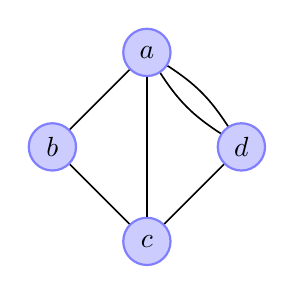
\begin{tikzpicture}[scale=1.2,node distance=3cm,semithick,inner sep=1pt,bend angle=45,auto]
%\draw[help lines] (-3,-3) grid (3,0);
\node[state]   (a) at  (90:1) {$a$};
\node[state]   (b) at (180:1) {$b$};
\node[state]   (c) at (270:1) {$c$};
\node[state]   (d) at   (0:1) {$d$};
\path
(a) edge (b)
    edge (c)   
    edge[bend left=12] (d)
	 edge[bend right=12](d)
(b) edge (c)
(c) edge (d);             
\end{tikzpicture}
\end{minipage}
%%%%%%%%
\begin{minipage}{0.45\textwidth}
\begin{tikzpicture}[scale=1.2,->,>=stealth',node distance=3cm,semithick,inner sep=1pt,bend angle=45,auto]
%\draw[help lines] (-3,-3) grid (3,0);
\node[state]   (a) at  (90:1) {$a$};
\node[state]   (b) at (180:1) {$b$};
\node[state]   (c) at (270:1) {$c$};
\node[state]   (d) at   (0:1) {$d$};
\path
(a) edge (d)   
    edge[loop above] (A)
(b) edge (a)
    edge (c)
(c) edge (a);             
\end{tikzpicture}
\end{minipage}
